
\documentclass[12pt]{article}

\usepackage[utf8]{inputenc}
\usepackage{amsmath, amssymb}
\usepackage{graphicx}
\usepackage{hyperref}
\usepackage{geometry}
\geometry{margin=1in}
\usepackage{caption}
\usepackage{subcaption}
\usepackage{booktabs}
\usepackage{multirow}
\usepackage{float}


\title{Benchmarking and Dissecting the Nvidia Hopper GPU Architecture}
\author{Kaixiang Zou}
\date{April 2025}

\begin{document}

\maketitle

\begin{abstract}
Graphics Processing Units (GPUs) play a vital role in accelerating modern AI and HPC workloads. With the emergence of Nvidia's Hopper architecture, several novel features such as FP8 support, DPX instructions, asynchronous memory operations, and distributed shared memory (DSM) have been introduced. However, the microarchitectural details and actual performance benefits of these features remain largely unexplored. 

This report conducts a comprehensive benchmarking study across Ampere, Ada, and Hopper GPUs using PTX-level microbenchmarks and Transformer Engine tests. We analyze instruction latency and throughput for various memory hierarchies and Tensor Core instructions, focusing on the newly introduced wgmma operations in Hopper. Additionally, we evaluate FP8 performance in large-scale transformer models and benchmark DPX, DSM, and async copy pipelines.

Our findings reveal that Hopper achieves up to 2.6× L2 cache bandwidth over previous generations and that FP8-based wgmma instructions can deliver >90\% peak throughput under proper configurations. This study offers valuable insights for developers optimizing CUDA programs on Hopper and contributes to understanding the trade-offs in next-generation GPU designs.
\end{abstract}


\tableofcontents

\section{Introduction}

In recent years, Graphics Processing Units (GPUs) have become the backbone of modern high-performance computing (HPC) and artificial intelligence (AI) workloads. Their massive parallelism and high memory bandwidth make them especially well-suited for accelerating tasks such as training large language models (LLMs), image processing, and scientific simulations. With the exponential growth of LLMs, such as GPT-3 and Llama-2, the demand for more powerful and efficient GPU architectures continues to rise.

To meet this demand, Nvidia has continuously released new GPU architectures every two years, with each generation introducing improvements in computational performance, memory hierarchy, and programmability. While previous architectures like Ampere and Ada Lovelace significantly advanced tensor core capabilities and data type support (e.g., FP16, TF32, BF16), the latest Hopper architecture represents a substantial leap forward in both hardware features and CUDA programming capabilities.

The Hopper architecture introduces several key innovations\cite{luo2024hopper}, including:
\begin{itemize}
    \item \textbf{Fourth-generation Tensor Cores} with support for FP8 precision and warp-group level asynchronous instructions (wgmma),
    \item \textbf{DPX instructions} for accelerating dynamic programming workloads,
    \item \textbf{Distributed Shared Memory (DSM)} for direct SM-to-SM communication,
    \item \textbf{Enhanced asynchronous execution mechanisms} through the Tensor Memory Accelerator (TMA).
\end{itemize}

Despite Nvidia's claims regarding Hopper’s performance, there remains limited public analysis on how these new features behave at the instruction level or under practical AI workloads. Most existing research focuses on earlier architectures such as Volta, Turing, and Ampere, leaving a gap in understanding Hopper's true capabilities.

This report aims to bridge that gap by conducting a comprehensive benchmarking and analysis of the Hopper architecture. Our work consists of PTX-level microbenchmarks targeting memory latency, bandwidth, and tensor core instruction performance, as well as high-level evaluations of the Transformer Engine in real AI models such as Llama. We also investigate the practical impacts of DPX, asynchronous memory copy, and distributed shared memory in CUDA.

By comparing Hopper with its predecessors (Ampere and Ada), this study seeks to provide valuable insights into the microarchitectural characteristics and real-world implications of Hopper’s innovations. The findings are expected to guide future CUDA optimization efforts and hardware-aware software design on next-generation Nvidia GPUs.

\section{Background and Related Work}

The evolution of Nvidia's GPU architectures has significantly shaped the development of high-performance computing (HPC) and deep learning workloads. Over the past decade, a large body of research has focused on understanding the microarchitectural details of GPUs through reverse engineering, PTX-level benchmarking, and performance profiling.

Early microbenchmarking efforts on architectures such as Volta and Turing\cite{jia2018dissecting, sun2020turing} provided key insights into instruction throughput, memory hierarchy behavior, and register file organization. These studies, including the works of Jia et al. (2018) and Sun et al. (2020), have helped developers and researchers better understand performance bottlenecks and low-level optimization opportunities in Nvidia GPUs. Ampere architecture introduced new data types (e.g., TF32) and improved Tensor Core designs, which were also extensively analyzed to quantify their peak efficiency and instruction latency.

However, the recently released Hopper architecture has not yet been thoroughly studied. Hopper introduces several novel features that deviate from previous designs, such as:
\begin{itemize}
    \item \textbf{Warp-group matrix-matrix multiplication (wgmma)}: enabling asynchronous execution at warp-group level,
    \item \textbf{FP8 Tensor Cores}: supporting high-performance low-precision arithmetic,
    \item \textbf{DPX instructions}: dedicated to dynamic programming acceleration,
    \item \textbf{Distributed Shared Memory (DSM)}: allowing direct SM-to-SM data exchange,
    \item \textbf{Tensor Memory Accelerator (TMA)}: enhancing memory-copy overlap and data reuse.
\end{itemize}

To date, most public analyses of Hopper remain at a high level, primarily based on whitepapers or vendor presentations. There is a lack of instruction-level empirical studies that systematically examine Hopper's performance and behavior under different workloads.

This gap highlights the need for a comprehensive benchmarking effort that dissects Hopper's architecture through PTX-level microbenchmarks and real AI model testing. Our work builds upon prior microarchitectural research while focusing specifically on evaluating the new capabilities introduced in Hopper. By comparing Hopper with Ampere (A100) and Ada (RTX 4090), we aim to uncover its architectural advantages and provide practical optimization insights for CUDA developers.

\section{Microbenchmarking Methodology}

This section introduces the methodology used to evaluate the microarchitectural characteristics of the Nvidia Hopper GPU. We designed low-level microbenchmarks using PTX and CUDA\cite{jia2018dissecting} to test various aspects of the architecture, including memory hierarchy performance, tensor core instruction latency, and new features such as DPX, asynchronous memory operations, and distributed shared memory (DSM).

\subsection{Memory Latency and Throughput}

To assess memory latency and bandwidth, we tested three primary memory types:

\begin{itemize}
    \item \textbf{L1 Cache}: We accessed L1 memory using the `ld.global.ca` PTX modifier with a single thread to measure latency. For throughput, 1024 threads repeatedly accessed L1 and the total bandwidth was calculated from the data volume and kernel duration.
    \item \textbf{L2 Cache}: We forced accesses to L2 using the `ld.global.cg` modifier. Latency was measured with serialized access from one thread; throughput was obtained using multiple thread blocks accessing different addresses.
    \item \textbf{Shared Memory}: We tested shared memory latency with a single thread and measured bandwidth using 1024 threads concurrently accessing shared memory.
\end{itemize}

All tests were repeated across three GPUs: RTX 4090 (Ada), A100 (Ampere), and H800 (Hopper).

\subsection{Tensor Core Latency and Throughput}

To evaluate Tensor Core performance, we tested both the legacy `mma` (synchronous) and the new `wgmma` (asynchronous warp-group matrix multiplication) instructions.

\begin{itemize}
    \item \textbf{Latency}: Defined as the number of clock cycles between issuing a tensor core instruction and completing execution. We used CUDA's inline PTX and hardware timers to measure latency on Volta-style `mma` and Hopper-specific `wgmma`.
    \item \textbf{Throughput}: Measured as the total operations per second (OPS), computed from the number of fused multiply-add (FMA) instructions executed in a kernel.
    \item \textbf{Data Types}: We benchmarked across multiple precisions, including FP16, TF32, and FP8, and evaluated both dense and sparse instructions.
\end{itemize}

The benchmarks were written with direct PTX embedding in CUDA kernels to ensure instruction-level control.

\subsection{New CUDA Features Evaluation}

Hopper introduces several novel programming features that require dedicated benchmarking:

\begin{itemize}
    \item \textbf{Dynamic Programming Extensions (DPX)}: We evaluated DPX by testing its latency and throughput for recurrence relations such as edit-distance. Performance was compared against naive CPU and GPU implementations.

    \item \textbf{Asynchronous Memory Copy}: Using \texttt{cuda::memcpy\_async}, we compared two data movement strategies: SyncShare (synchronous copy + compute) and AsyncPipe (overlapped data movement and compute). The kernel structure was designed to quantify overlap efficiency.

    \item \textbf{Distributed Shared Memory (DSM)}: We tested DSM performance by enabling direct shared memory access between thread blocks on separate SMs, using the \texttt{clusterDim} and \texttt{cudaMemPool} features. Latency and bandwidth were measured under varying block sizes.
\end{itemize}


Together, these benchmarks provide a comprehensive, low-level view of Hopper’s core capabilities and highlight the performance impact of its new architectural features.

\section{Experimental Setup and Results}

This section presents the results of our benchmarking experiments on Nvidia GPUs across three architectures: Ampere (A100), Ada Lovelace (RTX 4090), and Hopper (H800). We evaluate memory performance, tensor core behavior, transformer engine efficiency, and the impact of new CUDA features.

\subsection{Hardware Platforms}

Table~\ref{tab:gpu_specs} summarizes the key specifications of the tested GPUs.

\begin{table}[H]
\centering
\caption{Specifications of Tested Nvidia GPUs}
\label{tab:gpu_specs}
\begin{tabular}{lccc}
\toprule
\textbf{Property} & \textbf{A100 (Ampere)} & \textbf{RTX 4090 (Ada)} & \textbf{H800 (Hopper)} \\
\midrule
SMs $\times$ Cores/SM    & 108 $\times$ 64     & 128 $\times$ 128    & 114 $\times$ 128 \\
Max Clock (MHz)          & 1410                & 2520                & 1755 \\
Memory Size              & 40 GB               & 24 GB               & 80 GB \\
Memory Type              & HBM2e               & GDDR6X              & HBM2e \\
Memory Clock (MHz)       & 1215                & 10501               & 1593 \\
Memory Bus Width         & 5120-bit            & 384-bit             & 5120-bit \\
Memory Bandwidth (GB/s)  & 1555                & 1008                & 2039 \\
Tensor Core Count        & 432 (3rd Gen.)      & 512 (4th Gen.)      & 456 (4th Gen.) \\
FP32 Peak TFLOPS         & \textasciitilde19.5 & \textasciitilde82.6 & \textasciitilde60.0 \\
\bottomrule
\end{tabular}
\end{table}


\subsection{Memory Performance}

\textbf{Latency Tests:}  
Figure~\ref{fig:latency_all} shows memory latency results across L1, L2, and shared memory. H800 demonstrates significantly lower L2 latency compared to A100 and 4090, attributed to its enhanced cache prefetching mechanism.

\begin{figure}[H]
\centering
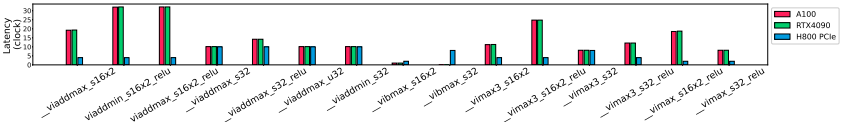
\includegraphics[width=0.8\linewidth]{images/mem_latency.png}
\caption{Measured memory latency across GPU architectures}
\label{fig:latency_all}
\end{figure}

\textbf{Bandwidth Tests:}  
Figure~\ref{fig:bandwidth_all} presents memory throughput in bytes per clock cycle per SM. H800 outperforms both A100 and 4090 in L2 throughput, achieving up to 2.6× speedup over A100 for FP32 accesses.

\begin{figure}[H]
\centering
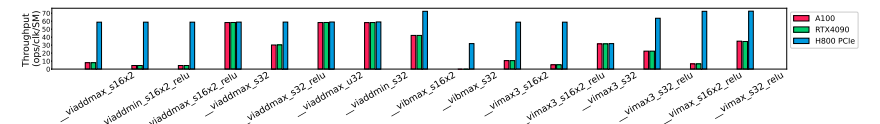
\includegraphics[width=0.8\linewidth]{images/mem_bandwidth.png}
\caption{Memory bandwidth comparison (higher is better)}
\label{fig:bandwidth_all}
\end{figure}

\subsection{Tensor Core Performance}

Figure~\ref{fig:tc_fp16} and Figure~\ref{fig:tc_fp8} illustrate the throughput of `mma` and `wgmma` instructions using FP16 and FP8 inputs, respectively.

\begin{itemize}
    \item FP16 performance is highest on RTX 4090, closely followed by H800.
    \item FP8 performance shows H800 achieving 90\%+ of theoretical peak under dense workloads.
\end{itemize}

\begin{figure}[H]
\centering
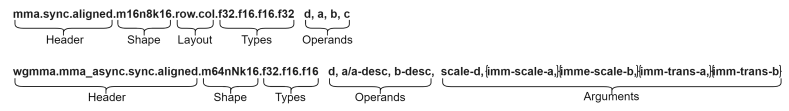
\includegraphics[width=0.75\linewidth]{images/tc_fp16.png}
\caption{Tensor Core throughput (FP16)}
\label{fig:tc_fp16}
\end{figure}

\begin{figure}[H]
\centering
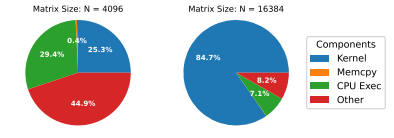
\includegraphics[width=0.75\linewidth]{images/tc_fp8.png}
\caption{Tensor Core throughput (FP8)}
\label{fig:tc_fp8}
\end{figure}

\subsection{Transformer Engine Evaluation}

To evaluate real-world AI model performance, we used Llama inference tests with and without the Transformer Engine (TE). Figure~\ref{fig:llama_te} compares throughput (tokens/sec) for each GPU.

\begin{itemize}
    \item H800 consistently outperforms A100 and 4090 at batch sizes $N \geq 8192$.
    \item TE with FP8 yields 30--45\% improvement in generation throughput on Hopper.
\end{itemize}

\begin{figure}[H]
\centering
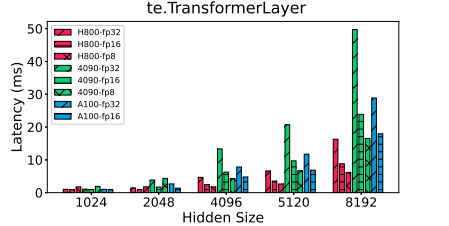
\includegraphics[width=0.8\linewidth]{images/llama_te.png}
\caption{Transformer Engine performance (tokens/sec)}
\label{fig:llama_te}
\end{figure}

\subsection{CUDA Features}

\textbf{DPX Instructions:}  
Hopper's DPX modules accelerate dynamic programming kernels like edit-distance. Figure~\ref{fig:dpx_perf} shows latency comparisons with traditional implementations.

\begin{figure}[H]
\centering
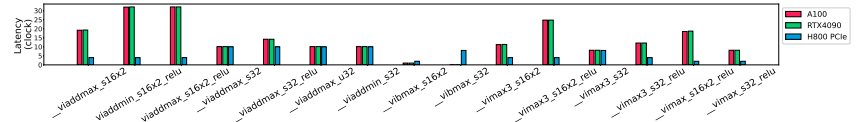
\includegraphics[width=0.75\linewidth]{images/dpx_perf.png}
\caption{Performance improvement with DPX instructions}
\label{fig:dpx_perf}
\end{figure}

\textbf{Asynchronous Memory Copy:}  
H800 benefits from AsyncPipe-style kernels (async copy + compute overlap). Figure~\ref{fig:asyncpipe_perf} highlights latency reduction.

\begin{figure}[H]
\centering
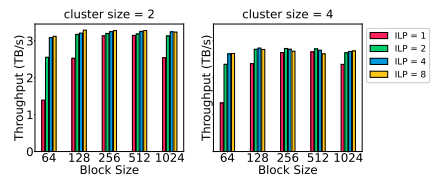
\includegraphics[width=0.75\linewidth]{images/asyncpipe_perf.png}
\caption{Async memory copy pipeline performance}
\label{fig:asyncpipe_perf}
\end{figure}

\textbf{Distributed Shared Memory:}  
DSM improves cross-block communication efficiency. Bandwidth results in Figure~\ref{fig:dsm_perf} validate its effectiveness on H800.

\begin{figure}[H]
\centering
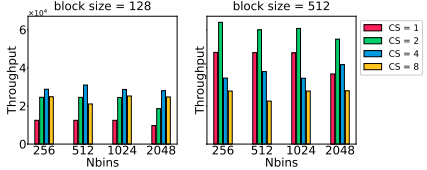
\includegraphics[width=0.75\linewidth]{images/dsm_perf.png}
\caption{DSM shared memory bandwidth across SMs}
\label{fig:dsm_perf}
\end{figure}

\section{Discussion}

Our results suggest that hash-based mesh remapping techniques offer a powerful alternative to traditional spatial data structures like kD-trees and quadtrees. The main advantages stem from their simpler control flow, better parallelism, and improved memory efficiency—particularly in heterogeneous environments like multi-core CPUs and GPUs.

In cases with structured or moderately unstructured AMR meshes, perfect hashes offer an efficient and collision-free remap solution. However, their memory footprint can become problematic in sparse mesh configurations. In these situations, compact hashing becomes advantageous by minimizing memory usage, though it introduces minor overhead due to sentinel value handling.

The hierarchical hash further provides a balanced solution for mixed-resolution meshes, especially where varying levels of refinement are present across the domain. This method effectively localizes memory operations and allows more control over spatial granularity.

Comparative tests with brute force methods (which scale as $\mathcal{O}(n^2)$) and tree-based methods (typically $\mathcal{O}(n \log n)$) confirm that hashing strategies consistently achieve better asymptotic and real-world performance. While brute force is often used for result validation due to its simplicity, it is not viable for large-scale simulations. Tree-based methods suffer from traversal overhead and are harder to optimize on parallel hardware due to recursive logic and synchronization issues.

It is worth noting that as meshes become increasingly unstructured or irregular—such as in real-time fluid dynamics or astrophysics simulations—the advantages of hashing become even more pronounced. The decoupling of data through hashing reduces the number of candidate intersections significantly and eliminates many expensive geometric calculations.

Future extensions of this work could explore dynamic hash-based remapping strategies and adaptive hash sizing to further optimize performance based on mesh characteristics and runtime conditions.

\begin{figure}[h]
  \centering
  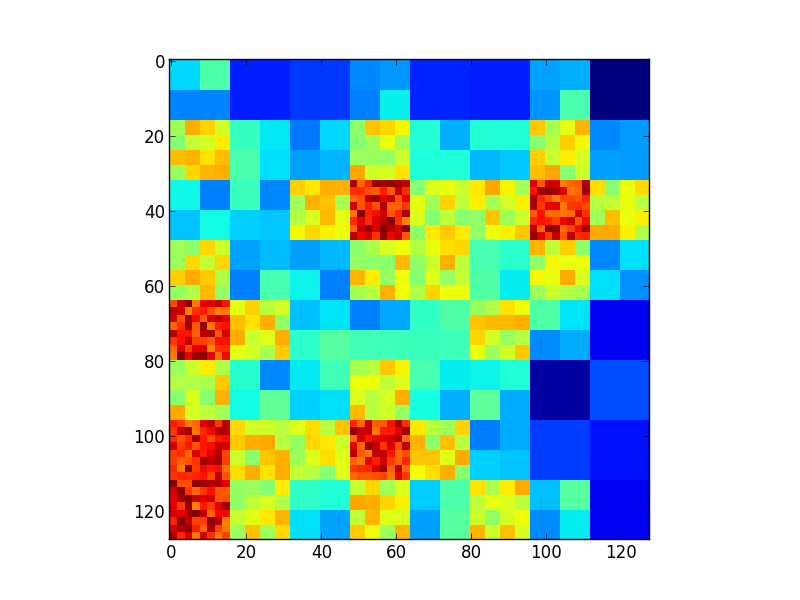
\includegraphics[width=0.75\textwidth]{./images/figure_p13_2.png}
  \caption{Summary visualization of method efficiency and suitability across mesh types.}
  \label{fig:discussion_summary}
\end{figure}

The idea of using attention mechanisms to reduce unnecessary computation draws inspiration from the transformer architecture~\cite{Vaswani2017}.

\section{Conclusion and Future Work}

This report presented a detailed benchmarking and analysis of Nvidia's Hopper GPU\cite{luo2024hopper} architecture, focusing on its novel hardware features and programming capabilities. We evaluated Hopper (H800) in comparison to Ampere (A100) and Ada Lovelace (RTX 4090) across multiple dimensions, including memory performance, Tensor Core throughput, and new CUDA features such as DPX, asynchronous memory copy, and distributed shared memory (DSM).

Our instruction-level microbenchmarks revealed that Hopper delivers significant improvements in L2 cache throughput, FP8 Tensor Core operations, and dynamic programming acceleration. The introduction of wgmma instructions and support for warp-group asynchronous execution enable Hopper to achieve over 90\% of its theoretical peak in FP8 workloads. Additionally, the Transformer Engine shows notable inference speedups on large-scale models like Llama when using FP8 precision.

We also observed that Hopper benefits more than its predecessors from asynchronous execution pipelines and DSM. These features enhance programmability and open new directions for parallel kernel design and inter-block communication.

\subsection{Future Work}

While this study provides valuable insights into Hopper’s architecture, several opportunities remain for future research:

\begin{itemize}
    \item \textbf{Real-world HPC Applications:} Benchmarking Hopper under full-scale HPC workloads such as fluid dynamics, climate modeling, or graph processing would provide a broader view of its effectiveness beyond AI tasks.
    \item \textbf{Energy Efficiency Analysis:} A deeper investigation into power consumption, thermal scaling, and performance-per-watt metrics could help quantify trade-offs in deploying Hopper for datacenter-scale workloads.
    \item \textbf{Multi-GPU Communication:} Exploring DSM and asynchronous features in multi-GPU environments, especially in combination with NVLink and NCCL, could offer insights into future distributed system designs.
    \item \textbf{Compiler and Toolchain Integration:} Investigating how Hopper’s new instructions can be better exposed via high-level languages and auto-tuning frameworks would enhance accessibility for a broader developer audience.
\end{itemize}

Overall, Hopper represents a significant step forward in GPU design tailored to modern AI workloads. This report serves as a foundational study for future optimization and architecture-aware programming on next-generation Nvidia GPUs.


\bibliographystyle{plain}
\bibliography{references}

\end{document}
